% Active research-report draft. The untouched supplied template is preserved
% in official_template.tex; the previous six-page attempt is in previous_version/.
\documentclass[journal,10pt,twoside]{IEEEtran}

\usepackage[utf8]{inputenc}
\usepackage[T1]{fontenc}
\usepackage{graphicx}
\usepackage{amsmath,amssymb,mathtools}
\usepackage{booktabs}
\usepackage{tabularx}
\usepackage{enumitem}
\usepackage{xcolor}
\usepackage{balance}
\usepackage{microtype}
\usepackage{dblfloatfix}
\usepackage{url}
\usepackage{pdfpages}
\usepackage[bookmarks=true,bookmarksopen=true]{hyperref}
\usepackage{cleveref}
\graphicspath{{images/}{../../docs/meetings/2026-10-19_update/figures/}}
\newcommand{\checkme}[1]{\textcolor{red}{[CHECK: #1]}}
\usepackage{natbib}% Force natbib.sty to put citation labels in the reference list
\makeatletter
\renewcommand\NAT@biblabel[1]{\def\citeauthoryear##1##2{##1 ##2}[#1]\hfill}
\renewcommand\NAT@bibsetup[1]{%
  \setlength{\itemsep}{\bibsep}\setlength{\parsep}{\z@}}
\def\@lbibitem[#1]#2{%
  \if\relax\@extra@b@citeb\relax\else
    \@ifundefined{br@#2\@extra@b@citeb}{}{%
     \@namedef{br@#2}{\@nameuse{br@#2\@extra@b@citeb}}}\fi
   \@ifundefined{b@#2\@extra@b@citeb}{\def\NAT@num{}}{\NAT@parse{#2}}%
   \item[\hfil\hyper@natanchorstart{#2\@extra@b@citeb}\@biblabel{#1}%
    \hyper@natanchorend]%
    \NAT@ifcmd#1(@)(@)\@nil{#2}}
\makeatother


\bibliographystyle{apalike}
\bibpunct{[}{]}{;}{a}{}{}

\setlist[itemize]{noitemsep,nolistsep,leftmargin=*}
\setlist[enumerate]{noitemsep,nolistsep,leftmargin=*}
\hypersetup{colorlinks=true,urlcolor=blue,linkcolor=blue,citecolor=blue}
\crefname{figure}{figure}{figures}
\Crefname{figure}{Figure}{Figures}
\crefname{table}{table}{tables}
\Crefname{table}{Table}{Tables}

\newcommand{\reporttitle}{Spatial Aware Peak Ranking in Mass Spectrometry Imaging}
\newcommand{\authorname}{Zayd \textsc{Suliman}}
\newcommand{\studentnumber}{2653934}
\newcommand{\supervisorname}{Hairong Bau and Richard Klein}
\newcommand{\academicyear}{2026}

\begin{document}

\title{%
  \vspace{4pt}
  
\includegraphics[width=0.12\textwidth]{images/witslogonew.png}\\[6pt]
  \Large\textbf{\reporttitle}%
}

\author{%
  \authorname,~Student~No.~\studentnumber\\
  \small School of Computer Science and Applied Mathematics,
         Faculty of Science, University of the Witwatersrand\\
  \small Supervisors:~\supervisorname \qquad \academicyear
}

\maketitle

\begin{abstract}
Mass spectrometry imaging (MSI) records thousands of mass-to-charge ($m/z$)
channels at every pixel of a tissue section, so analysis usually begins by
selecting a few informative peaks. Learned methods such as msiPL rank peaks
from an unsupervised model, and S\textsuperscript{3}PL adds spatial information through 3D
convolution. We ask whether local neighbourhood context improves learned peak
ranking and where in the pipeline it matters. Variational autoencoders with and
without neighbourhood input were segmented with a Gaussian mixture model.
Peaks were ranked either by Integrated Gradients (IG) through the model or by
correlating each ion image with the segment posterior maps. On 24 sections
from three public datasets, at matched peak budgets and under predeclared
decision rules, correlation outperformed IG in 140 of 144 paired comparisons
across three seeds, a difference that was statistically supported for every
dataset and model. In these tests, neighbourhood input to the encoder gave no
consistent, spatially specific gain, while spatially aware ranking statistics
were the strongest label-free rankings on two of the three datasets and within
0.01 of the best on the third.
\end{abstract}

\begin{IEEEkeywords}
mass spectrometry imaging, peak selection, variational autoencoder, spatial context, Integrated Gradients, reproducibility
\end{IEEEkeywords}

\section{Introduction}
\label{sec:introduction}

Mass spectrometry imaging (MSI) records a full mass spectrum at each location
of a tissue section, mapping many molecules at once without choosing targets in
advance~\citep{caprioli1997maldi,schwamborn2010molecular}. The data are large:
the sections used here have 972--4{,}761 measured pixels and 1{,}481--85{,}062
mass-to-charge ($m/z$) bins. Most analyses therefore begin by selecting a small
set of informative peaks. \emph{Peak picking} applies rule-based thresholds to
each spectrum and can discard weak but informative
ions~\citep{gibb2012maldiquant,lieb2020sparse}. \emph{Peak learning} instead
fits an unsupervised model and ranks $m/z$ bins by what the model uses.
Examples are msiPL, a variational autoencoder (VAE) on single
spectra~\citep{abdelmoula2021peak}, and S3PL, which adds spatial context through
3D convolution over tissue patches~\citep{weigand2026spatial}.

The proposal for this project, \emph{Representation Learning for Autonomous
Peak Detection in MSI}, set out to build \emph{Spatial-msiPL}: an msiPL-style
VAE given cheap local spatial context (the mean of a $3\times3$ neighbourhood),
as a lightweight alternative to 3D convolution. Testing it fairly raised a
second question: once a model is fitted, which part of the pipeline determines
peak quality? The candidates are the representation, the segmentation built on
it, and the attribution method used to rank bins.

We built Spatial-msiPL and its variants (uniform and attention-weighted
neighbourhoods, larger windows, masked centres) and segmented each latent space
with a Gaussian mixture model (GMM). Peaks were ranked by Integrated Gradients
(IG)~\citep{sundararajan2017axiomatic} of the GMM posteriors, or by directly
correlating each ion image with the posterior maps. All methods were scored at
matched peak budgets under rules fixed before the results, on 24 sections from
three public collections. The comparison included reproduced msiPL and S3PL
baselines and model-free rankings.

Holding the segmentation fixed, correlation outperformed IG in 136 of 140
paired comparisons across three training seeds, and this was statistically
supported in all six dataset--model comparisons. Neighbourhood input to the
encoder gave no consistent, spatially specific gain. Spatially aware
\emph{ranking} statistics, namely segmentation correlation and Moran's~$I$,
were the strongest label-free rankings. A linear PCA segmentation matched the
VAE. S3PL's published glioblastoma score lay outside ten reproduced seeds, and
weight initialisation switched individual S3PL sections between distinct
solutions.

The contributions are:
(i) a predeclared, matched-budget evaluation of learned MSI peak ranking on
three datasets;
(ii) a ranking ablation, with paired statistics, showing that
segment-then-correlate outperforms gradient attribution in this pipeline;
(iii) controlled tests that bound where spatial information helps;
(iv) a statistical account of S3PL's reproduction gap and seed sensitivity.
\Cref{sec:background} reviews related work, \cref{sec:questions} states the
research questions, \cref{sec:methodology} gives the methods,
\cref{sec:results} the results, \cref{sec:discussion} the discussion, and
\cref{sec:conclusion} concludes.

\section{Background and Related Work}
\label{sec:background}

\textbf{MSI data.} An MSI data cube has two spatial dimensions and one $m/z$
dimension~\citep{buchberger2018mass}. Spectra are usually normalised by total
ion current (TIC)~\citep{deininger2011normalization}. Neighbouring bins of one
molecular peak are strongly correlated, so a bin-level evaluation can reward
several bins of the same peak. This motivates the peak-level scoring used here.

\textbf{Learned peak selection.} msiPL trains a fully connected
VAE~\citep{kingma2014autoencoding} on single spectra and reads peaks from the
first-layer weights~\citep{abdelmoula2021peak}. massNet provides the GBM data
used here~\citep{abdelmoula2022massnet}. S3PL convolves over a spectral patch,
applies attention to the centre spectrum, reconstructs the whole patch, and
selects the bins with the most attention~\citep{weigand2026spatial}. It also
introduced the mask-based spatial-correlation F1 score (mSCF1), and reported
0.496, 0.601 and 0.470 on GBM, CAC and RCC, against 0.403, 0.431 and 0.159 for
msiPL. Other neural MSI work includes deep models of 3D
data~\citep{inglese2017deep} and ion-image
embeddings~\citep{guo2024deepion,weigand2026ionmorphnet}. Because S3PL changes
the architecture, objective, normalisation and selector together, it is
unclear which of them produces its gain, and whether much less spatial context
would suffice.

\textbf{Representation versus use.} Reconstruction quality need not predict
usefulness. \citet{mazarura2025autoencoder} found that reconstruction error,
cluster quality and downstream classification ranked autoencoders, PCA and NMF
differently on MSI data. We test the same distinction for peak ranking.

\textbf{Attribution and segment-then-correlate.} IG attributes a model output
to its inputs by integrating gradients from a baseline to the
input~\citep{sundararajan2017axiomatic}. Applied to a GMM posterior on a VAE
latent space, it ranks bins through the full nonlinear encoder. The older route
segments the tissue and correlates each ion image with the
segments~\citep{alexandrov2010spatial,alexandrov2011efficient}. Our pipeline
contains both on the same segmentation.

\textbf{Spatial statistics.} Moran's~$I$ measures spatial
autocorrelation~\citep{moran1950notes}. Spatial-structure measures have been
used to judge MSI ion images~\citep{alexandrov2013testing,cassese2016spatial},
and spatially aware segmentation smooths features with neighbourhood weights
before clustering~\citep{alexandrov2011efficient}.

\textbf{Gap.} Learned peak selectors are usually evaluated with unmatched peak
counts, single training runs and no model-free references. It has not been
tested under a common budget whether their advantage comes from spatial input,
the representation or the ranking step, nor how stable it is across seeds.

\section{Methodology}
\label{sec:methodology}

\subsection{Data}
\label{sec:data}
We used the three collections on which S3PL was published (\cref{tab:data}),
so that both baselines could be reproduced. GBM is the massNet patient-derived
xenograft (PDX) glioblastoma dataset (PR001292)~\citep{abdelmoula2022massnet}.
CAC is the MetaboLights colorectal adenocarcinoma dataset
(MTBLS415)\checkme{acquisition paper}. RCC comes from
\citet{dill2010rcc} via Cardinal~\citep{bemis2015cardinal}. The expert masks
come from the S3PL release~\citep{weigand2026spatial}.
\begin{itemize}
  \item \textbf{GBM:} sections from the same PDX line are not independent, so
        GBM is also summarised per line.
  \item \textbf{CAC:} all sections come from one biopsy, so its comparisons
        are within one specimen.
  \item \textbf{RCC:} cancer, normal and an unannotated region (45--78\% of
        pixels) are kept as three classes, with a cancer/normal-only
        sensitivity analysis.
\end{itemize}
Four sections (GBM108\_positive, GBM22\_2, 160TopL, 40TopL) were used for
development. RCC was held out until the method was frozen.

\begin{table}[t]
\caption{Datasets.}
\label{tab:data}
\centering\small
\begin{tabular}{@{}lccc@{}}
\toprule
 & GBM & CAC & RCC \\
\midrule
Sections & 8 & 8 & 8 \\
Independent units & 4 PDX lines & 1 biopsy & 8 subjects \\
$m/z$ bins & 85{,}062 & 1{,}481 & 10{,}200 \\
Pixels per section & 2{,}071--4{,}524 & 3{,}243--4{,}761 & 972--3{,}564 \\
Classes (GMM $K$) & 2 & 3 & 3 \\
\bottomrule
\end{tabular}
\end{table}

\subsection{Pipeline}
\label{sec:pipeline}
Each section is modelled on its own spectra without labels, and its selected
peaks are scored against its own masks. The design is unsupervised and
transductive. Masks never enter fitting or ranking, but they set two
configuration values, which are disclosed below.

\textbf{Spatial-msiPL.} Following msiPL, spectra are TIC-normalised and a fully
connected VAE (one hidden layer of 512 units, 5 latent dimensions) is trained
for 100 epochs with Adam (learning rate $10^{-3}$, batch size 128), using
msiPL's categorical cross-entropy reconstruction loss plus KL
divergence~\citep{abdelmoula2021peak}.
\begin{itemize}
  \item The \emph{centre-only} arm encodes one spectrum.
  \item The \emph{uniform} arm concatenates it with the mean of its up to eight
        measured $3\times3$ neighbours.
  \item Both reconstruct the centre only.
  \item The variants are learned attention over neighbours (about 0.5\% more
        parameters)~\citep{vaswani2017attention}, $5\times5$ to $9\times9$
        windows, zeroed and shuffled neighbours, and centre masking.
\end{itemize}

\textbf{Segmentation.} A full-covariance GMM is fitted to the standardised
latent means. Its number of components $K$ equals the number of annotated
classes, a class-informed choice that BIC did not support
(\cref{sec:res-encoder}).

\textbf{Rankings.} Each ranking orders the $m/z$ bins, and the top
$K_{\text{bin}}$ are scored.
\begin{itemize}
  \item \emph{IG}~\citep{sundararajan2017axiomatic} integrates the gradient of
        the assigned GMM posterior from the section-mean spectrum to 12 sampled
        pixels per component (64 trapezoidal steps), and ranks bins by mean
        absolute attribution, balanced across components.
  \item \emph{Posterior correlation} ranks bins by the absolute Pearson
        correlation of their ion images with each posterior map, balanced the
        same way, using the same GMM.
  \item \emph{Model-free references} are mean intensity, variance, Moran's~$I$
        over Moore-neighbour edges~\citep{moran1950notes}, and random.
  \item \emph{Ceiling:} a supervised oracle that correlates with the masks.
\end{itemize}
Test~V replaces the VAE with 5-component PCA, keeping the GMM and correlation
ranking. Test~S smooths the latent means with structure-adaptive weights before
the GMM~\citep{alexandrov2011efficient}.

\textbf{Baselines.} msiPL was reproduced and tuned to its published peak-count
procedure. S3PL was run from its public repository with the released settings:
10 epochs, Adam ($10^{-2}$), batch size 16, and patch size $p$ and peaks per
patch $z$ of 3/256 (GBM), 9/256 (CAC) and 5/1024 (RCC). The released code
normalises each patch by its spatial maximum, while the paper describes TIC
normalisation, so both were tested.

\subsection{Evaluation and design}
\label{sec:evaluation}
\textbf{mSCF1.} For each class mask and threshold
$t\in\{0.3,0.4,0.5,0.6\}$, a reference set of mask-correlated bins is formed
using the S3PL evaluator's rank cutoff. The F1 score between the selected bins
and the union of the reference sets is averaged over the four
thresholds~\citep{weigand2026spatial}. mSCF1 measures agreement with the
masks, not chemical identity.

\textbf{Budgets.} All compared methods select the same number of bins,
$K_{\text{bin}}$: the tuned msiPL count for GBM and CAC, and the released S3PL
target for RCC. A peak-level scale (P1) collapses neighbouring bins of one
mean-spectrum peak, so duplicates are not credited. On CAC and RCC, P1 is
nearly singleton and acts as a second budget check.

\textbf{Predeclared rules.} Every comparison's rule was written before its
outputs, in an append-only protocol.
\begin{itemize}
  \item A difference ``helps'' if its mean is at least $+0.02$ mSCF1 and it is
        positive in at least 6/8 sections.
  \item Two methods are ``equivalent'' if the mean difference is within
        $\pm0.02$.
  \item Otherwise the label is ``mixed'', or ``incomplete'' if sections are
        missing.
\end{itemize}
All arms use training seed~1. The two core arms were retrained with seeds 2
and~3 on all sections (Test~R). Seed results are given as mean~$\pm$~SD across
seeds of the seed-level collection means.

\subsection{Statistics}
\label{sec:stats}
The labels are accompanied by paired, per-section statistics:
\begin{itemize}
  \item the exact two-sided Wilcoxon signed-rank
        test~\citep{wilcoxon1945individual};
  \item the Hodges--Lehmann (HL) median difference with an exact 95\%
        CI~\citep{hodges1963estimates};
  \item the matched-pairs rank-biserial correlation $r$.
\end{itemize}
Seeds are averaged within section first. A Mann--Whitney test was not used,
because the comparisons are paired.

The 38 comparisons form five families by question: ranking (6), against
legacy msiPL (4), encoder variants (17), segmentation (9) and S3PL (2). Holm
correction~\citep{holm1979simple} is applied within each family. With $n=8$
the smallest possible $p$ is 0.0078, so only families of at most six tests can
reach Holm significance. Effect sizes therefore carry the main weight.

A result is ``statistically supported'' only if its Holm-adjusted $p<0.05$
\emph{and} its practical label agrees. GBM is also summarised per PDX line
($n=4$, smallest $p=0.125$). Mixed models with random section and seed effects
are descriptive.

\subsection{Computation}
\label{sec:compute}
Training ran on the University's Slurm cluster (RTX 3060 and 3090 GPUs), and
ranking ran on CPU nodes.
\begin{itemize}
  \item \textbf{Caching.} The original loader re-read every batch from HDF5 on
        shared storage. Data preparation took 24.6\,s per batch against about
        0.02\,s of computation, so a 100-epoch GBM run took 11.3\,h. Reading
        each section into memory once cut it to 23\,min ($30\times$), with
        identical losses and weights. The likely cause is repeated small network
        reads, but this was not separately measured.
  \item \textbf{Reuse of saved runs.} Same-seed reruns were checked to be
        bit-identical before any saved run was reused.
  \item \textbf{Timing.} Exact ranking equality depends on the CPU model, so
        timing runs used the processor type that produced each saved ranking.
\end{itemize}

\section{Results}
\label{sec:results}
Scores are mSCF1 at $K_{\text{bin}}$, seed~1, bin level, paired by section,
unless stated otherwise. Labels are quoted exactly.

\subsection{Baseline reproductions (RQ4)}
\label{sec:res-repro}
Each baseline was run under its own protocol and evaluator.
\begin{itemize}
  \item \textbf{msiPL} reproduced on all three collections: GBM 0.414 against
        0.403 published, CAC 0.402 against 0.431, and RCC 0.157 against 0.159.
  \item \textbf{S3PL} reproduced on CAC (0.592 against 0.601) and on RCC
        (0.41--0.44 over three seeds, against 0.47).
  \item \textbf{S3PL on GBM was not reproduced:} 0.32 against 0.496, using the
        current public code and released settings. The paper's supplementary
        settings were not available (\cref{sec:res-s3pl}).
\end{itemize}

\subsection{Correlation outperforms IG (RQ1, RQ2)}
\label{sec:res-main}
\Cref{tab:main} scores every ranking on the same segmentation and budget.

\textbf{Against msiPL.} Both VAE--IG arms beat reproduced msiPL in every GBM
and CAC section: 0.518 and 0.511 against 0.414 on GBM, and 0.528 and 0.560
against 0.402 on CAC. This is statistically supported in all four comparisons
(HL $+0.09$ to $+0.16$, Holm $p=0.031$). It compares whole pipelines, and one
predeclared clause (budget stability) could not be assessed.

\textbf{IG against correlation.} With the GMM held fixed, correlation with the
posterior maps beat IG in all 47 valid comparisons at seed~1
(\cref{fig:igcorr}). The predeclared rule's exact fall-through wording
applies: ``neither predeclared verdict applies, because IG scored below
posterior-$|$PCC$|$ in every section''. Over seeds 1--3, correlation won 136
of 140 comparisons (\cref{tab:seeds}).
\begin{itemize}
  \item The strict per-seed rule failed only at CAC seed~2, where IG was below
        in 6/8 sections instead of the required 7/8, so the label is ``does not
        hold overall''.
  \item No collection mean ever reversed direction.
  \item With seeds averaged within section, the difference is statistically
        supported in all six dataset--arm comparisons (\cref{tab:seeds}). Every
        section favours correlation ($r=-1$), and every raw $p$ is the
        smallest attainable for its $n$.
  \item The mixed models agree ($-0.24$ [$-0.27$, $-0.22$] on GBM, $-0.14$
        [$-0.17$, $-0.12$] on RCC) and attribute almost no variance to the seed.
  \item GBM is negative in every PDX line.
  \item Sampling 48 or 192 pixels for IG instead of 12 raised scores by at most
        0.024.
\end{itemize}
\emph{Answer:} the pipeline beats msiPL, but not because of IG. Given the same
segmentation, direct correlation is better on all three datasets. The useful
signal lies in the label-free segmentation.

\begin{table*}[t]
\caption{Collection mean mSCF1 at $K_{\text{bin}}$ (seed~1, bin level). All
rankings except the baselines use the same GMM. Bold: best label-free ranking.
The oracle uses the masks and is a ceiling.}
\label{tab:main}
\centering\small
\begin{tabular}{@{}llccccccccc@{}}
\toprule
Coll. & VAE arm & IG & Post.\ corr. & Moran's $I$ & Mean int. & Variance & msiPL & Random & Oracle \\
\midrule
GBM & centre & 0.518 & \textbf{0.743} & 0.684 & 0.483 & 0.497 & 0.414 & 0.009 & 0.809 \\
GBM & uniform & 0.511 & \textbf{0.744} & 0.684 & 0.483 & 0.497 & 0.414 & 0.009 & 0.809 \\
CAC & centre & 0.528 & 0.606 & 0.605 & \textbf{0.612} & 0.593 & 0.402 & 0.108 & 0.654 \\
CAC & uniform & 0.560 & 0.607 & 0.605 & \textbf{0.612} & 0.593 & 0.402 & 0.108 & 0.654 \\
RCC & centre & 0.412 & 0.568 & \textbf{0.631} & 0.498 & 0.508 & --- & 0.171 & 0.756 \\
RCC & uniform$^{a}$ & 0.410 & 0.596 & \textbf{0.635} & 0.499 & 0.504 & --- & 0.173 & 0.755 \\
\bottomrule
\multicolumn{10}{@{}l}{\footnotesize $^{a}$7 of 8 runs (UH0505\_12 failed the predeclared IG completeness check). msiPL on RCC is not budget-matched.}
\end{tabular}
\end{table*}

\begin{table}[t]
\caption{IG $-$ posterior correlation across seeds 1--3 (bin level): mean
$\pm$ SD of the seed-level collection means, wins for correlation, and paired
statistics on seed-averaged sections (HL with exact 95\% CI; Holm within F1).}
\label{tab:seeds}
\centering\scriptsize
\setlength{\tabcolsep}{3pt}
\begin{tabular}{@{}lcccc@{}}
\toprule
 & Mean $\pm$ SD & Corr.\ wins & HL [95\% CI] & Holm $p$ \\
\midrule
GBM centre & $-0.244 \pm 0.018$ & 24/24 & $-0.248$ [$-0.293$, $-0.186$] & 0.047 \\
GBM uniform & $-0.245 \pm 0.011$ & 23/23 & $-0.243$ [$-0.314$, $-0.159$] & 0.047 \\
CAC centre & $-0.077 \pm 0.003$ & 23/24 & $-0.078$ [$-0.116$, $-0.040$] & 0.047 \\
CAC uniform & $-0.055 \pm 0.007$ & 22/24 & $-0.046$ [$-0.080$, $-0.027$] & 0.047 \\
RCC centre & $-0.144 \pm 0.011$ & 22/23 & $-0.147$ [$-0.207$, $-0.082$] & 0.047 \\
RCC uniform & $-0.141 \pm 0.041$ & 22/22 & $-0.131$ [$-0.204$, $-0.056$] & 0.047 \\
\bottomrule
\end{tabular}
\end{table}

\begin{figure}[t]
\centering
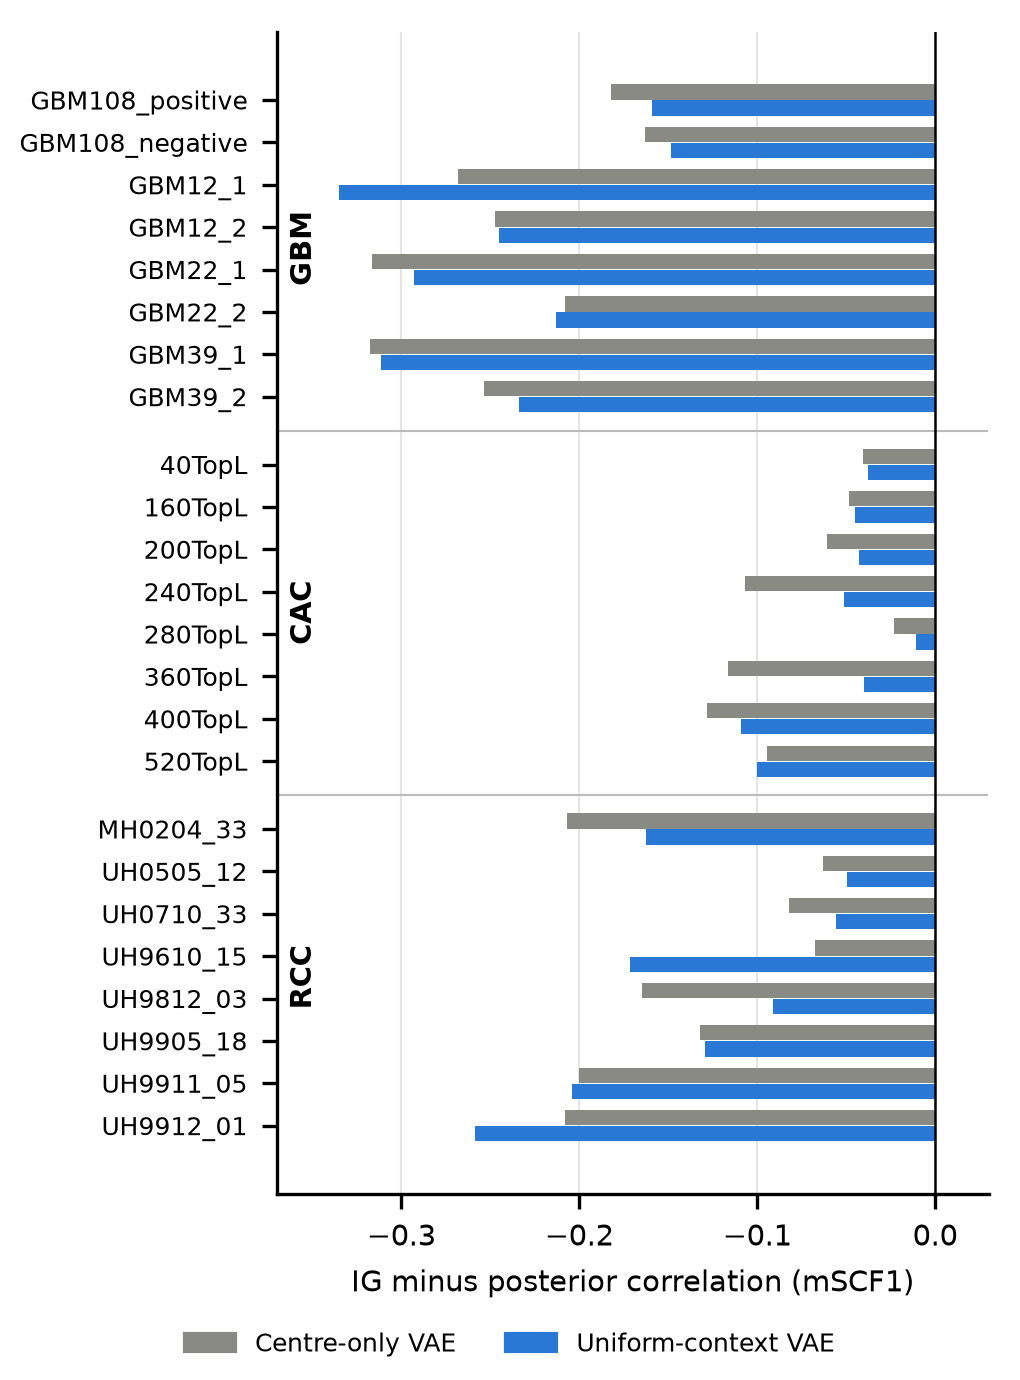
\includegraphics[width=\columnwidth]{05_ig_minus_correlation_by_section.png}
\caption{IG minus posterior correlation per section and VAE arm (seed~1). All
47 valid comparisons are negative.}
\label{fig:igcorr}
\end{figure}

\subsection{Simple rankings and the metric}
\label{sec:res-simple}
The best predeclared label-free ranking differs by dataset:
\begin{itemize}
  \item GBM: posterior correlation (0.743);
  \item CAC: mean intensity (0.612), with correlation, Moran's~$I$ and variance
        all within 0.02;
  \item RCC: Moran's~$I$ (0.63).
\end{itemize}
CAC is near saturation: every method, including the oracle, converges near
0.41 at twice the budget. On GBM and RCC, sections whose GMM matches the masks
better have correlation scores closer to the oracle (Spearman $\rho=-0.90$ and
$-0.84$). mSCF1 rewards ion images that follow the masks, so mask-like
segmentations score well when correlated against.

\subsection{Spatial context (RQ3)}
\label{sec:res-spatial}
\begin{itemize}
  \item \textbf{Uniform $3\times3$ context} ``helps'' IG on CAC ($+0.023$ over
        three seeds, 8/8 sections), but it is not statistically supported
        (Holm $p=0.13$) and is 0.000 under correlation ranking. On GBM the
        result is ``incomplete (7/8)'', with a mean of $+0.000$.
  \item \textbf{It is not spatially specific.} On CAC, real and shuffled
        nonlocal neighbours tied (0.542 against 0.543). On GBM, zeroed context
        scored highest.
  \item \textbf{Larger windows} ($7\times7$, $9\times9$) were $0.035$ below
        $3\times3$ on GBM (``mixed'') and ``equivalent'' on CAC.
  \item \textbf{Learned attention} was ``equivalent'' to uniform averaging
        ($+0.011$ GBM, $-0.006$ CAC). Its weights stayed near uniform with real
        neighbours (normalised entropy 0.98--0.999) but became selective with
        shuffled ones. The mechanism works; real neighbours are simply
        near-copies of the centre (median cosine about 0.98). Centre masking
        did not make attention selective and lowered GBM scores by 0.039.
  \item \textbf{Smoothed segmentation (Test~S)} was never labelled ``helps'':
        four ``equivalent'', one ``does not meet the `helps' rule (labelled
        mixed)'', and one ``incomplete''.
\end{itemize}
\emph{Answer:} spatial input to the encoder or the segmentation gave no
consistent, spatially specific gain. Spatial information helped as a ranking
statistic, through correlation with coherent segments and Moran's~$I$.

\subsection{Is the nonlinear encoder needed? (RQ2)}
\label{sec:res-encoder}
Replacing the VAE with PCA-5 while keeping the GMM and correlation gave VAE
$-$ PCA differences of $+0.023$ on GBM (5/8, ``mixed''), $-0.013$ on CAC
(``mixed'') and ``equivalent'' on RCC. These were unchanged with the VAE
averaged over three seeds. The VAE segmented slightly better (balanced
accuracy 0.868 against 0.839 on GBM) without reliably better peaks.

PCA-5 also had \emph{lower} reconstruction error than the VAE on all eight GBM
sections, and higher error on 7/8 CAC sections, so reconstruction did not
track peak quality~\citep{mazarura2025autoencoder}. BIC never validated the
number of components: it chose the largest candidate ($K=6$) every time.

\subsection{S3PL: neighbours, reproduction and seeds (RQ3, RQ4)}
\label{sec:res-s3pl}
\textbf{Neighbour dependence.} On CAC, retraining S3PL with every patch filled
with the centre spectrum collapsed it from 0.591 to 0.18 and 0.15 (two seeds,
8/8 sections). Shuffled nonlocal neighbours recovered most of the score (0.55
against 0.59), so correct placement added only about $+0.04$, inconsistently
(``mixed'', Holm $p=0.63$). Training for longer made S3PL worse: epoch 10 was
best in 15/16 sections.

\textbf{Reproduction gap.} Over ten released seeds (\cref{fig:s3plseeds}),
S3PL scored $0.319\pm0.042$ on GBM and $0.547\pm0.038$ on CAC.
\begin{itemize}
  \item \textbf{GBM:} the published 0.496 is about 4 SD above our mean. It is
        above every one of our seeds in 6/8 sections, and best-of-ten per
        section reaches only 0.434. Labels: ``outside our seed distribution''
        and ``not explained by seed selection alone''.
  \item \textbf{CAC:} the published 0.601 is just above our maximum (0.591),
        within its two-decimal rounding of best-of-ten (0.5998).
  \item \textbf{Normalisation:} switching to the TIC normalisation described in
        the paper did not raise GBM (0.303 against 0.324; HL $-0.012$
        [$-0.154$, $0.099$]), so it ``does not explain'' the gap.
\end{itemize}

\textbf{Why seeds matter.} About 52\% of the score variance is between
sections, 0--1\% is a seed main effect, and 47\% is a section $\times$ seed
interaction.
\begin{itemize}
  \item Seeds switch particular sections between distinct outcomes:
        GBM108\_positive moves between 0.02 and 0.46, and CAC 520TopL between
        0.17 and 0.71.
  \item The peak lists of different seeds can overlap by as little as 1\%.
  \item Varying only the weight initialisation, or only the data order, showed
        that initialisation dominated (SD 0.222 against 0.001 on
        GBM108\_positive), although order also mattered on GBM108\_negative.
  \item Same-seed reruns were bit-identical.
  \item Under TIC the per-section seed SD fell from 0.061 to 0.011.
\end{itemize}
\emph{Answer:} msiPL reproduces. S3PL reproduces except on GBM, where neither
seeds nor normalisation explain the gap. Its starting weights select between
distinct solutions, so single-seed comparisons against it are unreliable.

\begin{figure}[t]
\centering
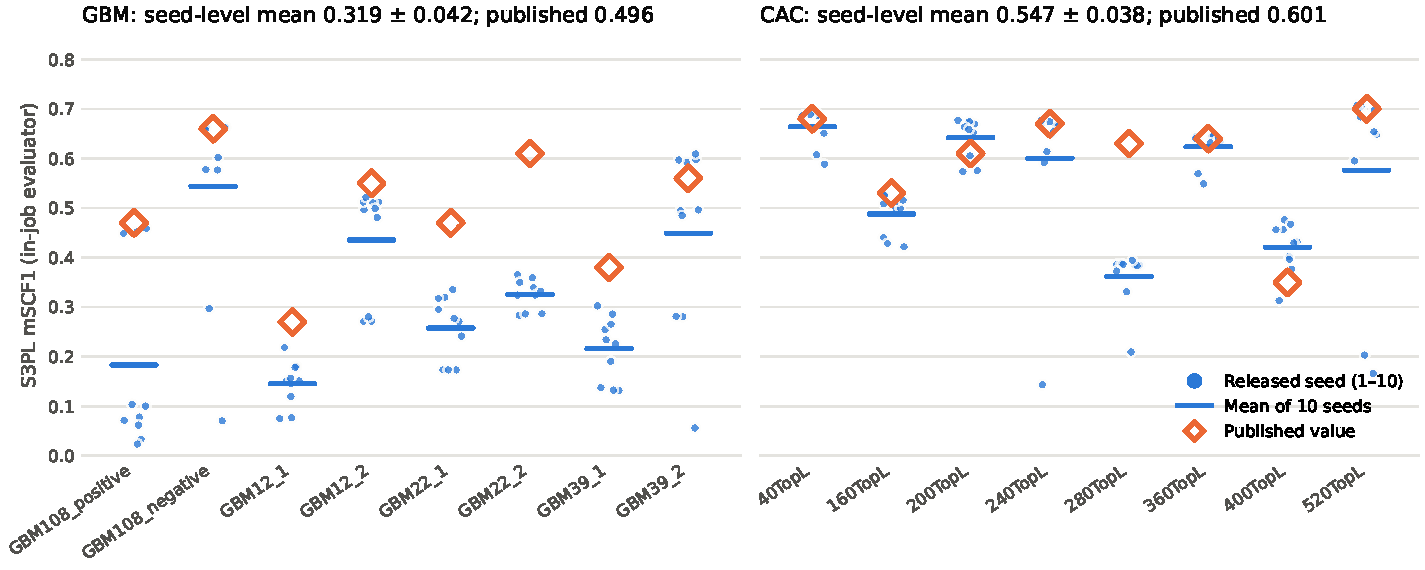
\includegraphics[width=\columnwidth]{s3pl_released_seed_distributions.pdf}
\caption{S3PL mSCF1 per section over ten released seeds (dots), the seed mean
(bar) and the published value (diamond), using S3PL's own evaluator.}
\label{fig:s3plseeds}
\end{figure}

\subsection{RCC and runtime}
\label{sec:res-rcc}
\label{sec:res-runtime}
\textbf{RCC.} On the held-out RCC data, correlation beat IG in every valid run
(0/8 and 0/7 positive), and Moran's~$I$ was the best label-free ranking. When
only cancer and normal pixels are scored, the advantage shrinks: correlation
beats IG in 5/8 runs (centre-only) and 6/7 (uniform). The three-class result
therefore partly reflects separating tissue from the unannotated region.

\textbf{Runtime.} Given a segmentation, correlation took 1.1\,s per GBM section
against 770\,s for IG (CAC 0.03 against 6.0\,s; RCC 0.11 against 372\,s), and
every timed ranking reproduced the saved ranking exactly.
\begin{itemize}
  \item Training: cached VAE runs took a median of 32--35\,min (GBM), 1.3\,min
        (CAC) and 2.2\,min (RCC), against 13.7, 0.9 and 1.6\,min for 10-epoch
        S3PL.
  \item Complete workflow, as the proposal planned to measure: on 160TopL the
        VAE took 122--135\,s against 151--174\,s for S3PL, with 1.2 against
        1.3\,GiB of RAM and 237 against 315\,MiB of GPU memory.
\end{itemize}
These are native-protocol measurements, not an equal-work comparison.

\section{Discussion}
\label{sec:discussion}

\subsection{Why correlation outperforms IG here}
Three explanations fit the ranking result.
\begin{enumerate}
  \item \textbf{Different questions.} IG asks which bins would change a few
        sampled pixels' component probabilities. Correlation asks which ion
        images follow a component across the whole section, which is closer to
        what mSCF1 rewards.
  \item \textbf{Sampling.} IG averages over 12 sampled pixels per component,
        while correlation uses every pixel. More pixels improved IG only
        slightly ($\le +0.024$) on the two sections tested, so sampling
        explains little of a gap of 0.05--0.25, but other IG settings
        (baselines, path counts, signed attributions) remain untested.
  \item \textbf{Metric alignment.} A segmentation that resembles the masks
        produces posterior maps that a mask-based metric naturally rewards.
\end{enumerate}
Correlation is therefore best read as an ablation finding about this pipeline:
the label-free segmentation carries the useful signal, and gradient attribution
through a dense VAE does not add to it. We do not claim that IG is generally
inferior, nor that segment-then-correlate, which is established
practice~\citep{alexandrov2011efficient}, is a new method.

\subsection{What remains of the spatial hypothesis}
The original hypothesis was that neighbourhood input would improve a VAE's
representation and therefore its peaks. In a dense VAE that averages or attends
over neighbours, no intervention gave a consistent gain beyond what nonlocal
(shuffled) context also provides, and smoothing the segmentation did not help
either. The attention experiments explain why. At $3\times3$ scale, adjacent
spectra are near-copies of the centre, so there is little to select between.
Spatially aware ranking statistics were strongest on GBM and RCC and within
0.01 of the best on CAC. S\textsuperscript{3}PL collapses without neighbour input
under its patch objective, although correctly placed neighbours added only an
inconsistent $+0.04$ over shuffled ones. These observations support a bounded
conclusion about the tested ranking statistics and encoder inputs.

\subsection{Reconstruction is not ranking quality}
PCA-5 reconstructed GBM better than the VAE yet ranked peaks about equally
well, while the VAE segmented slightly better. Earlier development runs showed
the same pattern: context models reconstructed slightly worse but changed which
peaks were chosen, and a spatial penalty smoothed the latents while worsening
reconstruction. Reconstruction error rewards fitting all intensity variation,
including intense ions unrelated to tissue classes, whereas peak quality here
depends on how well a low-dimensional segmentation separates the classes. This
agrees with \citet{mazarura2025autoencoder}.

\subsection{S\textsuperscript{3}PL instability and the reproduction gap}
The S\textsuperscript{3}PL seed analysis shows that comparisons with a single S\textsuperscript{3}PL run can be
misleading. Specific sections switch between distinct solutions depending on
the initial weights. The released preprocessing appears to create this
instability, since TIC normalisation removes it while also removing the
highest-scoring outcomes. Neither seeds nor normalisation explain the
published GBM score. We therefore report the gap as unresolved, and we do not
select favourable seeds or checkpoints for any baseline.

\subsection{Label-free operation and cost}
The pipeline fits and ranks without labels, but two settings still come from
annotation: the number of segments and the peak budget. BIC could not replace
the first, so the pipeline is not yet autonomous. On cost, the dense VAE used
comparable time and less memory than S\textsuperscript{3}PL on the section measured, and once a
segmentation exists, correlation ranking takes about a second where IG takes
minutes. The lightweight model is therefore practical, but it did not gain from
its spatial input, which was the reason for adding it.

\subsection{Limitations and threats to validity}
\begin{itemize}
  \item \textbf{Statistical units.} GBM has four PDX lines, CAC one biopsy and
        RCC eight subjects. P-values describe these sections, not a population.
        With $n=8$, only small families can reach Holm significance, so many
        comparisons rest on practical labels and effect sizes.
  \item \textbf{Class-informed configuration.} The number of GMM components
        equals the number of annotated classes and was not supported by BIC.
        Peak budgets come from published, annotation-related counts. The
        pipeline is label-free in fitting and ranking only.
  \item \textbf{The metric.} mSCF1 measures agreement with expert masks, not
        molecular identity. Methods that produce mask-like maps are favoured.
  \item \textbf{RCC.} The class-informed $K=3$ analysis partly reflects
        separating annotated tissue from an unannotated region that covers
        45--78\% of pixels. The Cardinal workflow treats this region as
        background, but that interpretation was not independently verified;
        two runs also have documented heterogeneous tumour.
  \item \textbf{Post hoc elements.} The PCA control, the smoothed
        segmentation, the seed replication and the S\textsuperscript{3}PL seed analysis were
        chosen after earlier results were known. Each was predeclared before its
        own outputs, and all are reported, including null and negative
        outcomes. Recommending correlation is a post hoc conclusion.
  \item \textbf{Scope.} The VAE uses fixed-window, dense neighbourhood input.
        Graph-based and ion-image-level spatial models, cross-section transfer,
        and other attribution settings were not tested.
\end{itemize}

\section{Conclusion}
\label{sec:conclusion}

This report tested whether local spatial context helps a lightweight VAE
select informative MSI peaks, and which part of a learned pipeline determines
peak quality. Under matched budgets and predeclared rules, on three public
collections, we reached the following conclusions.
\begin{itemize}
  \item Ranking peaks by correlation with a label-free GMM segmentation
        outperformed gradient attribution through the VAE on every dataset.
        This was statistically supported and stable across training seeds.
  \item Neighbourhood input to the encoder and smoothing of the segmentation
        gave no consistent, spatially specific gain. Spatially aware ranking
        statistics were strongest on GBM and RCC and within 0.01 of the best
        on CAC.
  \item A linear PCA segmentation performed comparably to the VAE, and
        reconstruction error did not track peak quality.
  \item msiPL reproduced. S\textsuperscript{3}PL's published GBM score did not.
        Weight initialisation dominated seed sensitivity in two of three
        selected sections, while data order also mattered in one.
\end{itemize}

The contribution is a controlled evaluation, not a new peak picker. It shows
how spatially aware rankings performed in these datasets, and how
strongly conclusions depend on fair budgets, model-free references and seed
replication.

Future work should first:
\begin{itemize}
  \item validate a label-free choice of the number of segments, which BIC
        could not provide;
  \item test a predeclared combination of segmentation correlation and
        Moran's~$I$ on new data;
  \item evaluate spatial models that operate on graphs or whole ion images
        rather than fixed windows;
  \item test whether a model fitted on one section transfers to another.
\end{itemize}


\section*{Acknowledgements}
The author thanks Hairong Bau and Richard Klein for their supervision and
guidance, and the University of the Witwatersrand for access to the MSCluster
computing facility.

\bibliography{references}

\clearpage
\onecolumn
\IfFileExists{ai_declaration.pdf}{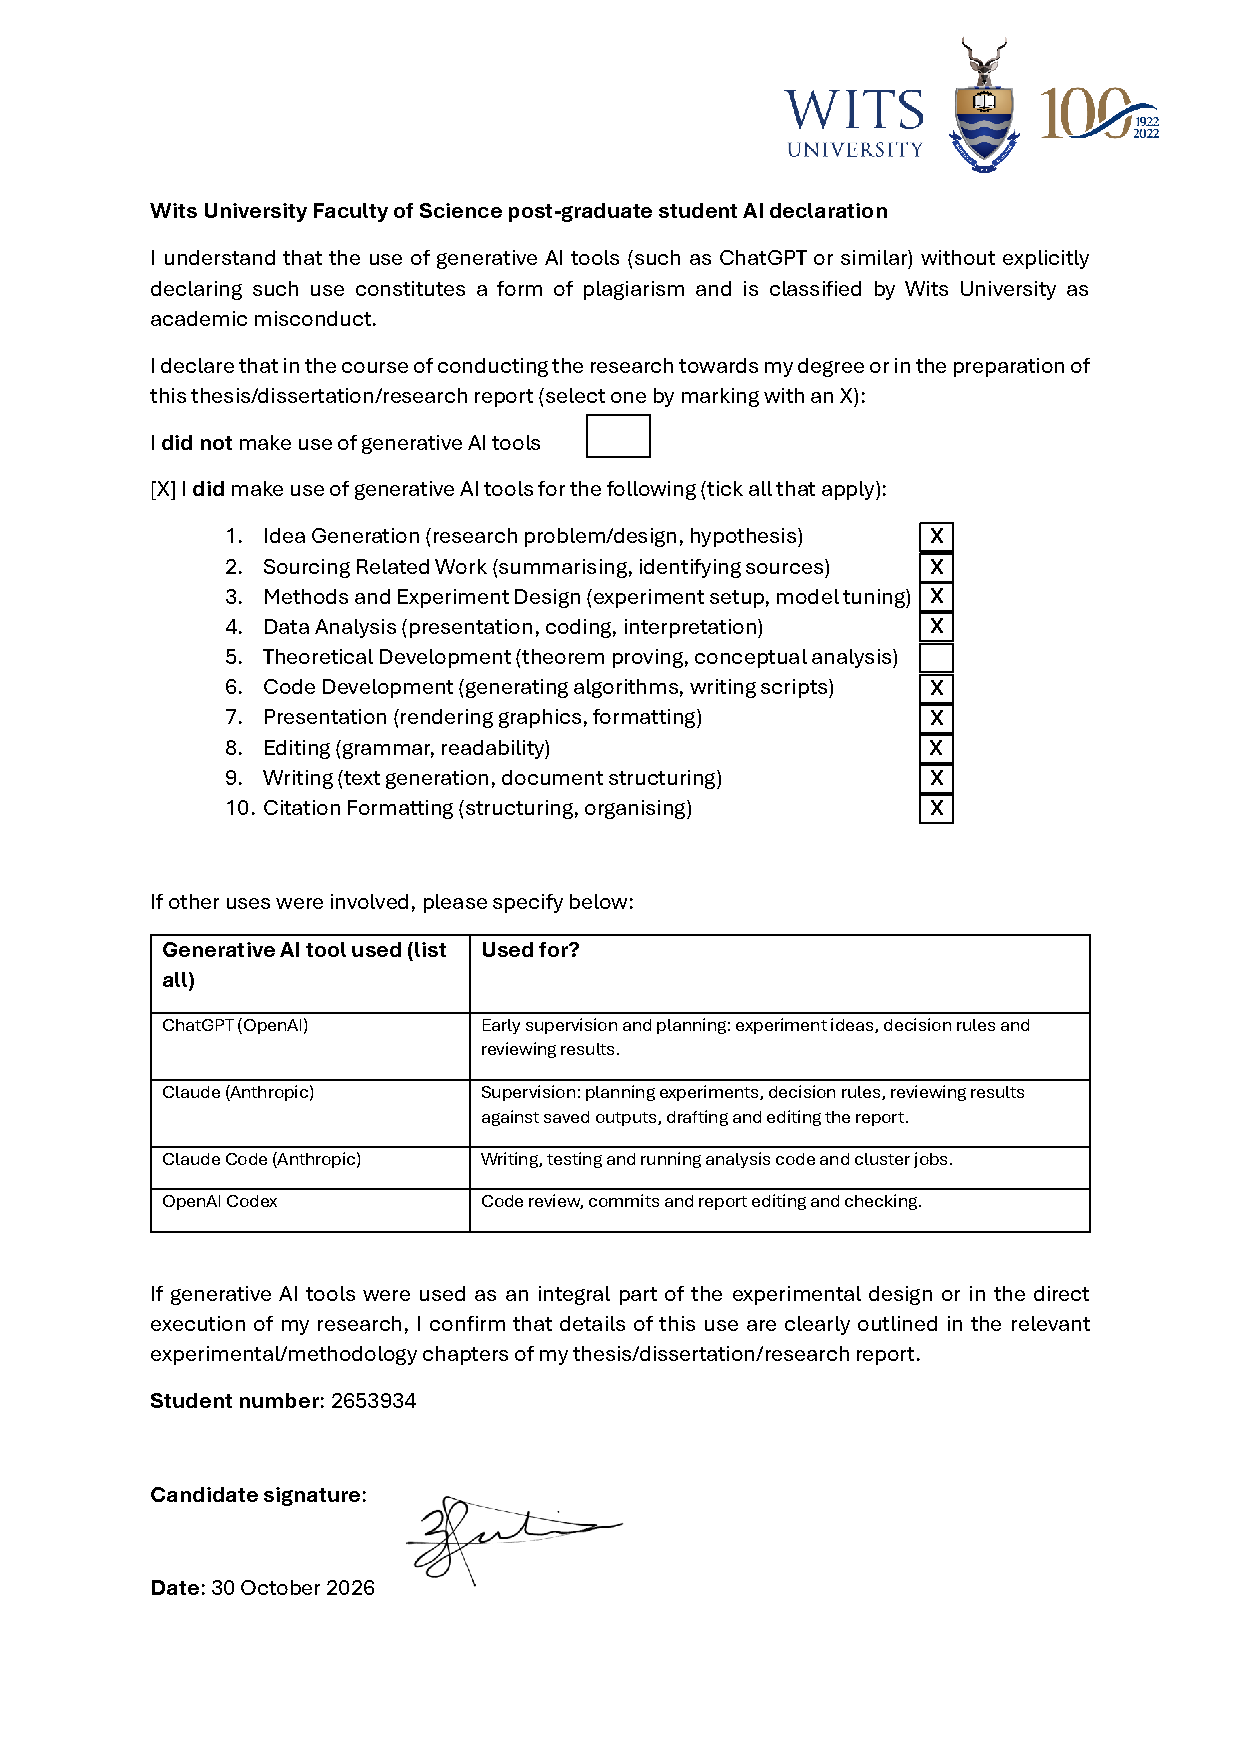
\includepdf[pages=1]{ai_declaration.pdf}}{%
\section*{AI declaration}
\checkme{Completed Wits postgraduate AI declaration form (final page), with
the tools used and the relevant prompts on additional pages.}}
\end{document}

